\documentclass[12pt]{article}
\usepackage[left=1in, right=1in, top=1in, bottom=1in]{geometry}
\usepackage{graphicx}
\usepackage{url}
\usepackage{cite}
\usepackage{float}
\usepackage{caption}
\usepackage{subcaption}
\usepackage{hyperref}
\hypersetup{
    colorlinks,
    citecolor=black,
    filecolor=black,
    linkcolor=black,
    urlcolor=black
}

\renewcommand{\familydefault}{\sfdefault}


\begin{document}
\begin{titlepage}
    \begin{center}
        \LARGE
        \textbf{ELE 402 - GRADUATION PROJECT II}
        
        \Large
        \textbf{TERM REPORT}
        
        \vspace{70pt}
        
        \textit{
            Hacettepe University \\
            Department of Electrical and Electronics Engineering
        }
    \end{center}
    
    \vspace{90pt}
    
    \large
    
    \textbf{Project Title:} Sensor Fusion in the Cloud \\
    
    \textbf{Project Group Members:} Ertuğrul Tiyek, Ahmet Yusuf Şirin
    
    \vspace{30pt}
    
    \textbf{Project Supervisor:} Asst. Prof. Dr. İsmail Uyanık \\
    
    \textbf{Submission Date:} 18.06.2023
    
    \vspace{\fill}
    
    \begin{center}
        \textit{FALL 2022-2023}
    \end{center}
\end{titlepage}

\clearpage

\tableofcontents
\listoffigures
\listoftables

\clearpage

\begin{abstract}
    Our project centers around sensor fusion, a critical aspect of artificially perceiving and enhancing the environment. By leveraging sensors, computers can acquire data on diverse environmental parameters. While each sensor has its strengths and weaknesses, even sensors designed for different purposes can contribute to augmenting the same information. Our project specifically focuses on extracting depth information through sensor fusion techniques, including EKF, CNN, and a novel iterative algorithm inspired by Papoulis Gerchberg. This algorithm operates in the frequency domain, reducing the processing workload compared to per-pixel control algorithms. The depth information obtained through our approach holds tremendous potential for a wide range of applications, including autonomous vehicles, UAVs, augmented reality devices, and 3D modeling. Additionally, we explore the integration of cloud computing to meet the computational demands of complex control algorithms or neural networks, ensuring accurate depth estimation. Our work places particular emphasis on the utilization of legged robots and highlights the significance of reliable odometry data extraction for simultaneous localization and mapping (SLAM).
\end{abstract}


\section{INTRODUCTION}

This report provides an overview of the completed project, which focuses on sensor fusion and SLAM operations within a fully ROS-based robot. The project aimed to develop an autonomous robotic platform capable of mapping and navigating its environment using a diverse set of sensors. The previous interim report outlined the prototype design, iterations, and evaluation results. In this final report, we will discuss the progress made since the interim report, including the additional work carried out. One significant accomplishment is the development of our sensor fusion algorithm, which has been further accelerated through the implementation of CUDA libraries. Cloud computing was also integrated into the project, and a modular Docker container structure was adopted to enhance system independence and scalability. Additionally, the SLAM process was performed using various algorithms and real-time as well as recorded datasets. Overall, this report presents a comprehensive overview of the project's accomplishments, including the development of the sensor fusion algorithm, cloud computing integration, SLAM implementation, and adherence to engineering standards and design constraints. The subsequent sections will delve into the specific details of each aspect, providing a comprehensive understanding of the completed project. 


\section{PROJECT DESCRIPTION}

Our project focuses on the development of a fully autonomous robotic platform that utilizes sensor fusion and SLAM techniques to navigate and map its environment. The primary objective is to create a robust system capable of perceiving and augmenting the surrounding environment by combining data from various sensors. By leveraging sensor fusion algorithms such as EKF, CNN, and an iterative approach inspired by Papoulis Gerchberg, we aim to extract accurate depth information. 

The extracted depth information holds significant potential for a wide range of applications, including autonomous vehicles, unmanned aerial vehicles (UAVs), augmented reality devices, and 3D modeling. To handle the computational demands of complex control algorithms and neural networks for precise depth estimation, we explore the integration of cloud computing. This allows us to leverage high computing power and achieve enhanced accuracy. 

Our project incorporates the use of legged robots, which offer increased mobility and adaptability in diverse environments. Additionally, reliable odometry data extraction is emphasized, as it plays a crucial role in simultaneous localization and mapping (SLAM). By ensuring accurate odometry, we can effectively construct and update a map of the unknown environment while keeping track of the robot's location within it. 

Modularity, system independence, and scalability are crucial considerations for our project. To achieve these goals, we have implemented a Docker container structure that facilitates easy integration and maintenance of the system components. This approach allows for seamless expansion and upgrades as needed. 

Throughout the project, we have made significant advancements in sensor fusion, algorithm development, cloud computing integration, and SLAM implementation. The combination of these elements forms a comprehensive robotic platform capable of autonomously navigating, perceiving, and mapping its surroundings. Our project not only demonstrates the practical application of sensor fusion and SLAM but also provides valuable insights and a foundation for future developments in the field.


\section{ENGINEERING STANDARDS AND DESIGN \\ CONSTRAINTS}

\subsection{ENGINEERING STANDARDS}

Several engineering standards were followed throughout the project to ensure efficient and reliable communication, interoperability, and data transmission between the various components of the robotic system. These standards include: 

\begin{itemize}
    \item TCP/IP (Transmission Control Protocol/Internet Protocol):
          
          The SSH (Secure Shell) protocol, based on TCP/IP, was used for secure communication between internal computers of the robot. It provides encrypted data transmission, ensuring confidentiality and integrity. 
          
    \item UDP (User Datagram Protocol):
          
          UDP was utilized for transmitting Lidar data. UDP is a lightweight and connectionless protocol, well-suited for real-time applications where low latency is crucial. 
          
    \item ROS (Robot Operating System):
          
          ROS was employed as the communication framework for transmitting stereo camera information and facilitating communication between different modules of the system. ROS provides a standardized messaging protocol, allowing seamless integration of various sensors and modules. 
          
    \item Wi-Fi 802.11.ax:
          
          The Wi-Fi 802.11.ax standard was utilized for wireless communication. This standard offers high-speed, reliable wireless connectivity, enabling communication between the robotic platform and external devices. 
\end{itemize}

Adhering to these engineering standards ensures compatibility, efficient data transmission, and secure communication within the robotic system. By employing TCP/IP, UDP, ROS, and Wi-Fi 802.11.ax, the project meets industry best practices for communication protocols, enabling seamless interaction between components and modules of the robot. 


\subsection{DESIGN CONSTRAINTS}

From the "Project Design Constraints" document, our constraints are:

\begin{itemize}
    \item \textbf{Economy:} \\
          For the term project duration we have no spending other then the supervisors did. In case of further production, maintenance, we should spend around 18 dollars without counting the costs of the work put forward. We cannot find this such project on the market. But educational project like ours exist.
          
    \item \textbf{Environment:} \\
          Our robot is battery powered and now on it is only in the development process by different cases. Hence for now we do not have any power consumption calculations (also because we are focused on the software). The radiation we uncovered are on the ISM RF band, legally. And there is no serious pollution of noise, hopefully.
          
    \item \textbf{Manufacturability:} \\
          Physical implementation will consist of collecting materials and combining them due to use of ready made products. Since, there is no need for high level technologies of manufacturing.
          
    \item \textbf{Sustainability:} \\
          If we look at the reliability and durability of the design, we can say the legged robot that we use is waterproof but there are a few of external components those are not. Our project is a comprehensive study in which the mathematical foundations of a product that can serve humanity in many areas such as personal use, industrial use and use in disasters are laid and upper engineering problems are solved. In this way, its sustainability is high because it sits on a very comprehensive basis. Also upgrades for scaling purposes are possible to implement since the software we are developing has an abstraction from the hardware. 
          
\end{itemize}

and the other constraints for our project specifically due to usage of the some bought products are:

\begin{itemize}
    \item \textbf{Computing Power}
          \begin{itemize}
              \item \textbf{Internal Nvidia Jetson Nano 4GB:} \\
                    Mobile computing devices tend to have less computing power due to their size limits. There are three Nvidia Jetson Nano devices inside of the Unitree Go1 Edu. These devices located in the robot to perform certain tasks. Two of Nvidia Jetson Nano 4GB and one Nvidia Jetson Nano 2 GB development kits are used for getting data from camera and sensors, processing raw data to extract dept information of stereo cameras, human skeleton tracking and so on. 
                    
                    We don’t need most of the features of the robot like human tracking in our project, so we can lighten its workload and use one of them as our computing unit. 
                    
              \item \textbf{External Nvidia Jetson:} \\
                    In case of having a trouble with using internal Nvidia Jetson device, we can also use an external one. It can be again a Nvidia Jetson Nano with all resources dedicated to our sensor fusion algorithm or a more advanced model like Xavier Nx. This option will rise the cost of the project, so this is an option only if actually needed. 
                    
              \item \textbf{Cloud Computing:} \\
                    Computing is any goal-oriented activity requiring, benefiting from, or creating computing machinery~\cite{enwiki:1120224488}. There are different computing elements. CPU’s have ability to work high clock frequencies and have large set of sequential instructions. GPU’s are mostly  Mobile computing devices like Nvidia’s Jetson series development kits may not match the performance requirements in some cases. There are GPU servers to provide high parallel computing power.
                    
          \end{itemize}
          
          \vspace{10pt}
          
          \begin{table}[H]
              \centering
              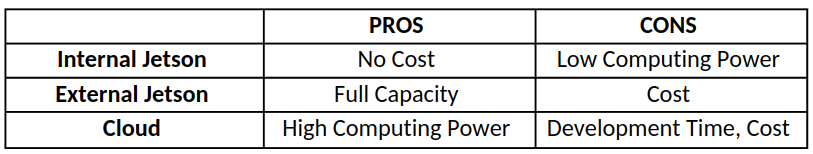
\includegraphics[width=0.8\textwidth]{ComputerComparison.png}
              \caption{Computing Power Comparison}
          \end{table}
          
          \textbf{Result:}
          
          We decided to use Internal Jetson Development kits of the robot for sake of cost reduction. But as mentioned before, one of the aims of this project is moving execution of algorithms that need high computing power to the cloud. So, we will be using both internal Jetson devices and cloud computing. That will be give us an opportunity to compare results in both alternatives. 
          
    \item \textbf{Depth Sensor \& Stereo Camera}
          \begin{itemize}
              \item \textbf{Internal Unitree Camera – Super Sensory System:} \\
                    Lens Angle ~150°×170° 
                    
                    \begin{figure}[H]
                        \centering
                        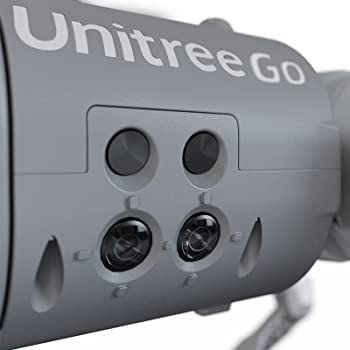
\includegraphics[width=0.5\textwidth]{SuperSensorySystem.png}
                        \caption{Super Sensory System}
                    \end{figure}
                    
              \item \textbf{External ZED Stereo Camera:} \\
                    
                    \begin{figure}[H]
                        \centering
                        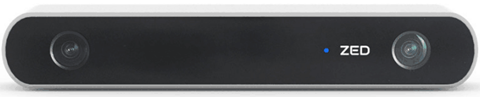
\includegraphics[width=0.5\textwidth]{ZEDCam.png}
                        \caption{ZED Stereo Camera~\cite{ZEDStereoCamera}}
                    \end{figure}
                    
                    Some specifications of ZED: 
                    
                    \begin{itemize}
                        \item High-Resolution and High Frame-rate 3D Video Capture (1080p 30fps)
                        \item Depth Perception indoors and outdoors at up to 20m
                        \item 6-DoF Positional Tracking
                        \item Spatial Mapping
                        \item 110° Wide Angle Cameras
                    \end{itemize}
                    
              \item \textbf{Xbox 360 Kinect:} \\
                    \begin{figure}[H]
                        \centering
                        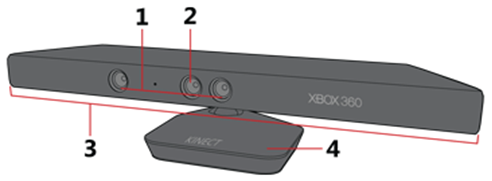
\includegraphics[width=0.5\textwidth]{XBoxKinect.png}
                        \caption{Xbox 360 Kinect~\cite{XboxKinect}}
                    \end{figure}
                    
                    \begin{enumerate}
                        \item 3D Depth sensor (IR Emitter + IR Camera / Depth Sensor)
                        \item RGB camera (Color Sensor)
                        \item Microphone array
                        \item Tilt motor (for detecting floor and players in the play space)
                    \end{enumerate}
                    
              \item \textbf{Velodyne 80-VLP-16-A 3D LiDAR:} \\
                    \begin{figure}[H]
                        \centering
                        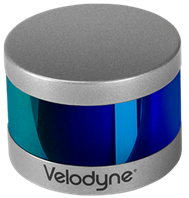
\includegraphics[width=0.3\textwidth]{LiDAR.png}
                        \caption{Velodyne LiDAR}
                    \end{figure}
                    
                    Some specifications of LiDAR:
                    
                    \begin{itemize}
                        \item 100 m Range
                        \item 360° x 30° Viewing Angle
                        \item 0.3 Million Points/Second
                        \item 100Mbps Ethernet \& UDP Interface
                        \item Rated IP67
                    \end{itemize}
          \end{itemize}
          
          \vspace{10pt}
          
          \begin{table}[H]
              \centering
              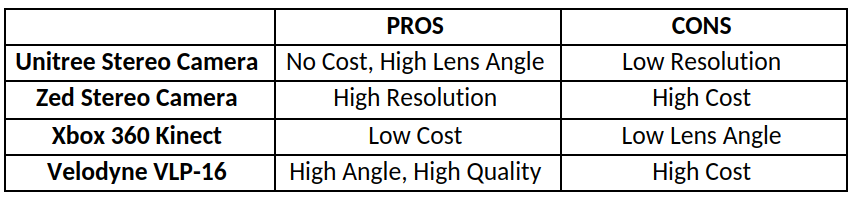
\includegraphics[width=0.8\textwidth]{SensorProsCons.png}
              \caption{Sensor Comparison}
          \end{table}
          
          \textbf{Result:}
          
          As we consider the trade-offs that are given at table-x, we decided to move on with Unitree Stereo Cameras and Velodyne VLP-16 3D Lidar. 
          
    \item \textbf{Programming Languages} \\
          There are different tools we need to use to control the robot, access its sensor measurements and camera data etc. The robot manufacturer provides SDKs to access and control the robot. These SDKs are implemented using C++ programming language. 
          
          There is an SDK provided by Unitree to control robots with software. The SDK is implemented in C/C++ languages, but it supports programming in C, C++ and Python languages. So, at some point, we had to use those languages. 
          
          Besides these, ROS technology has a lot of programming languages provided. Since, we have no restriction from this side, hopefully. 
          
          \vspace{10pt}
          
          \textbf{Result:}
          
          As we consider the performance and easy usage, we are planning to use Python only for algorithm development. After that we will be implement same algorithms in C++ to improve performance. SDK handles most of the ROS work, but we use ROS commands if it needed. 
          
\end{itemize}


\section{SUSTAINABLE DEVELOPMENT GOALS}

Our project is a comprehensive study in which the mathematical foundations of a product that can serve humanity in many areas such as personal use, industrial use and use in disasters are laid and upper engineering problems are solved. In this way, its sustainability is high because it sits on a very comprehensive basis. If we look at our project in the context of global goals, it is a good example of Goal 9: Industry, Innovation, and Infrastructure. In addition, our design successfully complies with Goal 12: Responsible consumption and production, as abstractions are kept neatly. For example, scaling in design using the same software infrastructure is quite possible and simple.


\section{BACKGROUND}

For this project the need of strong background is irrefutable. Since there is software oriented design for our case, the reasearchs are more leading. Background comes from the earlier courses in our department, additional research, professional life, and even daily life. Also tricky parts are coming from experiences of our supervisors (know-hows, etc.).

\subsection{BACKGROUND ACQUIRED IN EARLIER COURSE WORK}

The sensor fusion operation require a lot mathematical theory and its practical implementations. At this point, the importance of our Calculus (MAT123/124) and Engineering Mathematics (MAT235/236), Signals and Systems (ELE301), Control Systems (ELE354), and Digital Signal Processing (ELE407) courses takes place. 

But they are not enough to come up with a practical project. To design the system of this large computing environment and the network we should lay on the Computers and Programming (ELE107), Computer Programming (ELE118/120), Data Structures (ELE411), and Data Communication (ELE412) courses. For the sensor fusion operation we also use the knowledge from the Image Processing (ELE492) course for filtering bases and the hands-on programming purposes.

\subsection{BACKGROUND ACQUIRED THROUGH ADDITIONAL\\ RESEARCH}

Although our courses that we took in our department are pretty important for the theoretical base and introductory for the implementation, the know-hows of the programming languages, computer architectures, design patterns, and the protocols that we use are beyond from the course curriculums. To get those knowledge, we made a lot of research about those. Besides this, specifically the programming language practices are coming from our part-time jobs, internships, extracurricular studies, and further studies, and coding practices which coming from our supervisors suggestions.

To be more specific, the CPP and the Python programming languages are not taught but we should already know those to go further in our design. Another example is ROS (robot operating system) concept that is special for our purposes has nothing to do with our courses. Sensor fusion is also a specific research area of the digital signal processing, control systems, mathematics, and Computer Vision~\cite{enwiki:1120271364} for ur case, obviously. Hence, we also made lots of preliminary study in this topic, other than courses.


\section{METHODS}

The definition of our project is explained in detail in the first interim report. In the light of the definition, we try to make the decisions and the design parameters clear. To sake of easiness we draw some paths going same destination and arguing to reach the optimal path on the alternatives. Those alternatives are listed and described below. Then we will clearly elucidate our method now.

Since the project includes plenty of areas to work those are distinct, we divide them into subtopics. Those are:

\begin{enumerate}
    \item Sensor Choosing Methods
    \item Sensor Fusion Methods
    \item Sensor Data Enhancement Methods
    \item Fusion Data Enhancement Methods
\end{enumerate}

\subsection{Sensor Choosing Methods}

Our aim in this project is to achieve high reliability by using (fusing) all the sensors we have together. However, when we want to do all these together, we foresee that the project will reach very different dimensions. Therefore, while continuing the project, we decided to select a number of sensors in order to focus on algorithm development.

We set ourselves criteria when choosing sensors. Easy to use sensors is one of our main priorities due to our job description. In addition, considering the algorithmic complexity, working with sensors with linear system response is also an important criterion. In addition, the frequency of receiving data from the sensor is of great importance. Because if the sensor data we will fuse does not come at the same frequency, we will need to add operations to our algorithm to make the sensor frequencies equal by upsampling and downsampling.

We basically divided the sensors we have into two groups as those producing RGBD data or those producing Depth Point Cloud data.

\subsubsection{Method 1: Internal Sensor Using}
The internal sensors of the legged robot include five pairs of stereo cameras that produce RGBD data, and ultrasonic sensors that produce Depth Point Cloud data when viewed cumulatively, SuperSensorySystem. In addition to these, each foot has pressure sensors and an internal IMU.

\subsubsection{Method 2: External Sensor Using}
Our external sensors are ZED Stereo camera which produces RGBD data, Velodyne 3D LiDAR which produces Depth Point Cloud data and Xbox 360 Kinect having 3D depth sensor, RGB camera, microphone array, and also tilt motor. In the future, it is also possible to add sensors such as IMU and GPS to support odometry information.

\subsubsection{Method 3: Mixed Sensor Using}
We can also use our sensors mixed. However, complexity will increase in this method and the workload to be done before the sensor fusion algorithm will become more.


\begin{itemize}
    \item \textbf{Internal Unitree Camera – Super Sensory System:} \\
          Lens Angle ~150°×170°
          
          \begin{figure}[H]
              \centering
              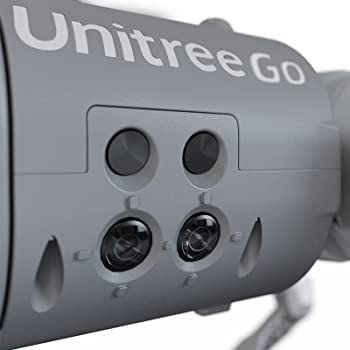
\includegraphics[width=0.5\textwidth]{SuperSensorySystem.png}
              \caption{Super Sensory System}
          \end{figure}
          
    \item \textbf{External ZED Stereo Camera:} \\
          
          \begin{figure}[H]
              \centering
              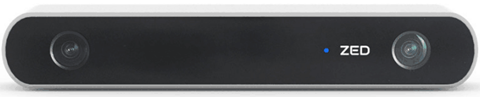
\includegraphics[width=0.5\textwidth]{ZEDCam.png}
              \caption{ZED Stereo Camera~\cite{ZEDStereoCamera}}
          \end{figure}
          
          Some specifications of ZED:
          
          \begin{itemize}
              \item High-Resolution and High Frame-rate 3D Video Capture (1080p 30fps)
              \item Depth Perception indoors and outdoors at up to 20m
              \item 6-DoF Positional Tracking
              \item Spatial Mapping
              \item 110° Wide Angle Cameras
          \end{itemize}
          
    \item \textbf{Xbox 360 Kinect:} \\
          \begin{figure}[H]
              \centering
              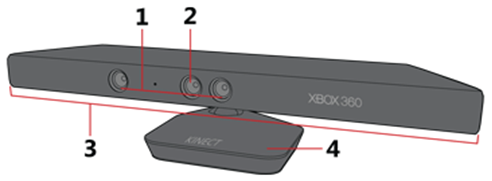
\includegraphics[width=0.5\textwidth]{XBoxKinect.png}
              \caption{Xbox 360 Kinect~\cite{XboxKinect}}
          \end{figure}
          
          \begin{enumerate}
              \item 3D Depth sensor (IR Emitter + IR Camera / Depth Sensor)
              \item RGB camera (Color Sensor)
              \item Microphone array
              \item Tilt motor (for detecting floor and players in the play space)
          \end{enumerate}
          
    \item \textbf{Velodyne 80-VLP-16-A 3D LiDAR:} \\
          \begin{figure}[H]
              \centering
              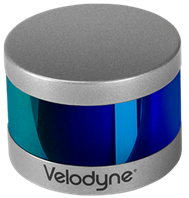
\includegraphics[width=0.3\textwidth]{LiDAR.png}
              \caption{Velodyne LiDAR}
          \end{figure}
          
          Some specifications of LiDAR:
          
          \begin{itemize}
              \item 100 m Range
              \item 360° x 30° Viewing Angle
              \item 0.3 Million Points/Second
              \item 100Mbps Ethernet \& UDP Interface
              \item Rated IP67
          \end{itemize}
\end{itemize}

We have taken all these into consideration while doing the preliminary design, and together with the evaluations under the following headings, we have determined a starting point for ourselves. You can find the details under the Preliminary design heading.

% Stereo Camera Decision Method
% LiDAR Decision Method
% Internal IMU usage on legged robot
% Documentation about sensors in marketplace and we owned (engineering decisions on costs)


\subsection{Sensor Fusion Methods}

\subsubsection{Method 1: Complementary Filter}
We wanted to set out using known methods for sensor fusion. In this way, we aimed to improve the performance we want to achieve with methods that we understand fundamentally, instead of using the resources in the literature directly. In fact, we started out by examining the usages of Kalman filter and extended Kalman filter, which are quite commonly used for state estimations made from aircraft IMU sensors, in this field. We predicted that if you continue on your way by choosing the most primitive complementary filter among them, we will be able to understand more clearly that we are moving away from the target in every development we make.

\begin{figure}[H]
    \centering
    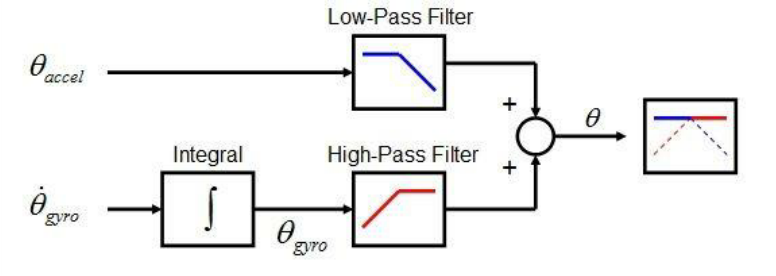
\includegraphics[width=0.7\textwidth]{CF.png}
    \caption{Complementary Filter Example for Aircraft Attitude}
\end{figure}

\subsubsection{Method 2: Kalman Filter}
Using the Kalman filter is also a method between using the extended Kalman filter and using a complementary filter. Since we want to use it with some methods that will enhance compelemntery filtery, we have already produced our own gain function. However, we also considered the Kalman filter as a method.

\begin{figure}[H]
    \centering
    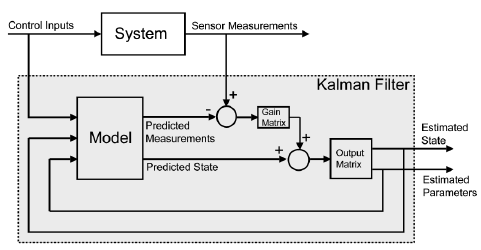
\includegraphics[width=0.7\textwidth]{KF.png}
    \caption{Kalman Filter Example for Aircraft Attitude}
\end{figure}

\subsubsection{Method 3: Extended Kalman Filter Method}
In addition to previous methods, we also evaluated the opinion that preliminary design can speed up the process by directly using the most advanced extenden Kalman filter. However, unlike in the aircraft scenario, we could not find an example use for depth data to be suitable for our scenario~\cite{9307398}.

\begin{figure}[H]
    \centering
    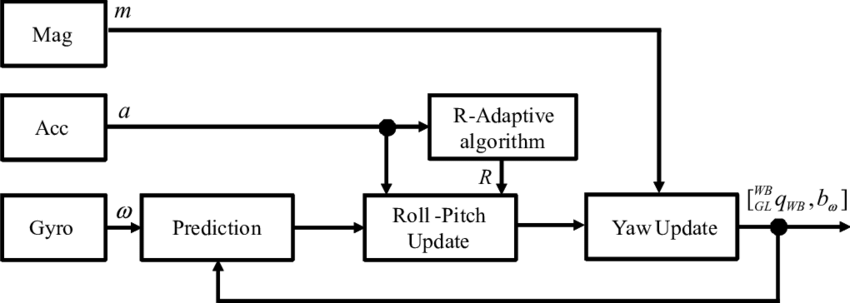
\includegraphics[width=0.7\textwidth]{EKF.png}
    \caption{Extended Kalman Filter Example for Aircraft Attitude}
\end{figure}

A comparison in which the models in which the state estimator methods are effective and the noise characteristics are given together is given in the X table, cost function comparisons for further analysis~\cite{The_cost_function_of_the_data_fusion_process_and_i}.

\begin{table}[H]
    \centering
    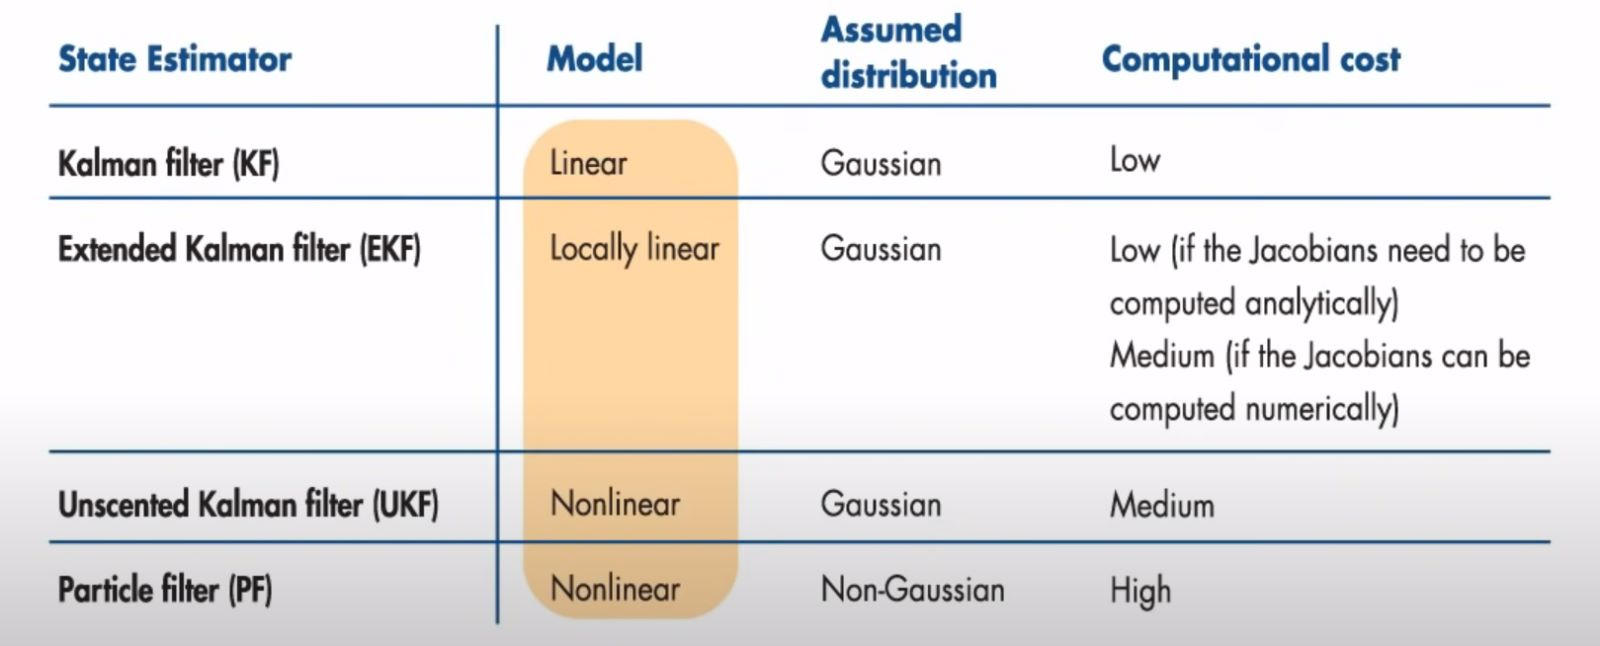
\includegraphics[width=0.8\textwidth]{CostComparison.jpeg}
    \caption{Cost Function Comparison}
\end{table}


\subsection{Sensor Data Enhancement Methods}

We compare the following methods for data enhancement to following data fusion.

\subsubsection{Method 1: Only Data Rate and Range Matching}
Since the data we want to obtain is odometry, we evaluated creating parametric inputs in the methods we used while continuing the project. Because we sould think about Sensor Data Rate - State Estimation Relation. In this way, we aimed to analyze whether we could establish a relationship between the quality of the raw data and the esimated odometry data. After some tests we will briefly report our results about early sensor data enhancement for sensor fusion.

\subsubsection{Metod 2: Papoulis-Gerchberg Algorithm for Depth Point Cloud}
We are searching about Papoulis-Gerchberg algorithm effects on LiDAR and Stereo depth map results to enhance the data resolution before data fusion. An image super-resolution method, the Papoulis–Gerchberg (P–G) algorithm, on range data represented in the form of a greyscale image. However, the low convergence rate of the original P–G algorithm impedes its use for online applications~\cite{ozbay2015high, kuzucu2018enhancing}. By referencing this method we also proposed as an enhancement method.~\cite{6280128}


\section{PRELIMINARY DESIGN}

ZED stereo camera and Velodyne 3D LiDAR were chosen for the preliminary design, which are sensors that are well-documented, have a large community, and are easier to use and access resources than the internal sensors of the legged robot. This sensor will also minimize the complexity of the algorithm to be used in sensor fusion, as they offer a wide resolution and data rate band.

As the sensor fusion algorithm, it was ordered from simple to complex or from low to high performance, and it was decided to make a start with a complementary filter. Again, it was decided to use methods such as edge preservation~\cite{9307398} as an aid to the main algorithm in order to increase the sensor fusion performance.

We choose the complementary filter for fusing the depth information of two sensors. Each sensor has its own properties, advantages and disadvantages. According to these characteristics of sensors we tune our sensor fusion algorithm. But like all control systems, we first regulate our input signals to work with.

Thing we have to match in these two sensors data is viewing angle. Stereo vision camera has a viewing angle upto 110°. We simply reduced the viewing angle of the 3D lidar to match the stereo vision cameras viewing angle. But further steps we are planning to use also 360° lidar information to enhance environmental data while performing SLAM.

Raw data provided by lidar and stereo vision cameras in different formats. Stereo vision camera extracts depth frames as well as RGBD (Red Green Blue Depth) in cartesian form. 3D lidar extracts data in point cloud form which is basically in spherical form. In the other hand the resolution of stereo vision data is available in 2208x1242 at 15 fps, 1920x1080 at 30fps, 1280x720 at 60 fps, 672x376 at 100 fps. The 3D lidar works completely different and samples much less data. In order to match the sampled data from two sensors, we decided upsampling the lidar data and converting it to cartesian form. We use dynamic Papoulis–Gerchberg algorithm to augment the lidar data and then linearly interpolate this information while converting point cloud data to depth frame.

Iterative Papoulis–Gerchberg algorithm is the method used to recover the lost samples of the signal. It is mostly used for super resolution images in image processing. In a single frame manner, iterative Papoulis–Gerchberg algorithm will be enough to increase data in a single point cloud of a lidar. But our aim is continuously matching the frames, we will use the dynamic Papoulis–Gerchberg algorithm. This algorithm make use of stillness of background and continuity of movement to reduce computational effort in Papoulis–Gerchberg.

There is also difference between sample rates of two sensors. Stereo camera samples frames in range of 15 to 100 frames per second. Lidar samples point clouds by rotating its lidar continuously. Each rotation provides one whole 360° sample (30° vertical). Lidar works in range 300 rpms to 600 rpms. That provides us 5-to-10 point clouds per second. We aim to up-sample the  number of point cloud per second by again linear interpolation.

There is one more problem with the lidar. Ability of lidar is not limited by the only rotation but also sample rate of sensor. Increasing rotation speed reduces the quality of the point clouds. One part of the project is experiencing the different data rates and calculating the processing effort, transmission capabilities and response times. So we will optimize resolution and data rates in the content of this project.

\subsection*{Sensor Fusion Algorithm}

We matched the formats of the input signals to keep the sensor fusion simple. There are two depth images as input signals to get more accurate depth image.

As a preliminary design, we are planning to calculate the depth image in per pixel fashion. As mentioned before, the complementary filter is formulated as:

\begin{equation}
    \hat{x} = \hat{x}_1 \alpha + \hat{x}_2 (1 - \alpha)
\end{equation}

We will generate $\alpha$ generation function to calculate $\alpha$ for each pixel and condition. Input sources are not functioning perfect in every conditions. There are some internal and external variables that effects the accuracy of measurement. Let’s observe these variables:


\subsubsection*{Variables That Effect Lidar:}

\begin{itemize}
    \item Beam Angle:
          
          3D lidar scans the environment in a three-dimensional manner. Velodyne VLP-16 scans 360° horizontally and 30° vertically. In different beam angles, Lidar accuracy depends. There is an article that contains more information about beam angle effect.
          
          \begin{figure}[H]
              \centering
              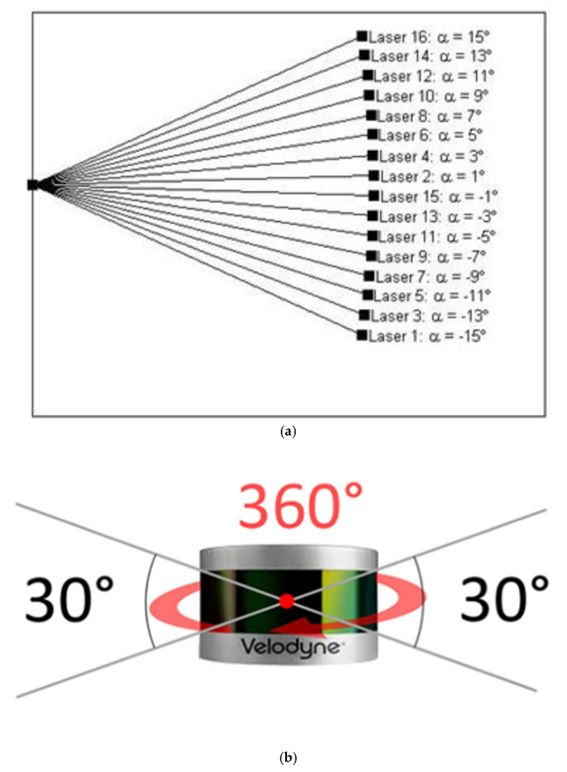
\includegraphics[width=0.5\textwidth]{LidarAngles.jpeg}
              \caption{Velodyne LiDAR Beam Angles~\cite{VelodynePerformance}}
          \end{figure}
          
    \item Rotation Speed:
          
          Sample rate of the lidar decreases as rotation speed of the lidar increases. It effects the quality of the depth image. But increasing the rotation speed provides us approximation to real time application.
          
    \item Distance:
          
          3D lidars can work in a range that is specified in datasheet. Out of this range, lidar cannot work properly. As we think of the working principle of the lidar, the processing time is not enough to measure too close points. The Velodyne VLP-16 model has a working range between 1m to 100m.
          
    \item Rough and Uneven Views:
          
          The Lidar is using wavelengths very close to visible light to observe visible objects. In some environments like forests, rough areas, rainy and foggy weathers there are lots of indentations like branches, twigs and leaves or water drops. Each of this bits and pieces prevents the infrared laser lights coming from lidar and creates canopies. Instead of a clean point cloud, lidar gets a noisy one.
          
          We can measure the effect of the bits and pieces in the environment to accuracy of lidar measurement by calculating the gradient of depth frame around target pixel.
          
          \begin{figure}[H]
              \centering
              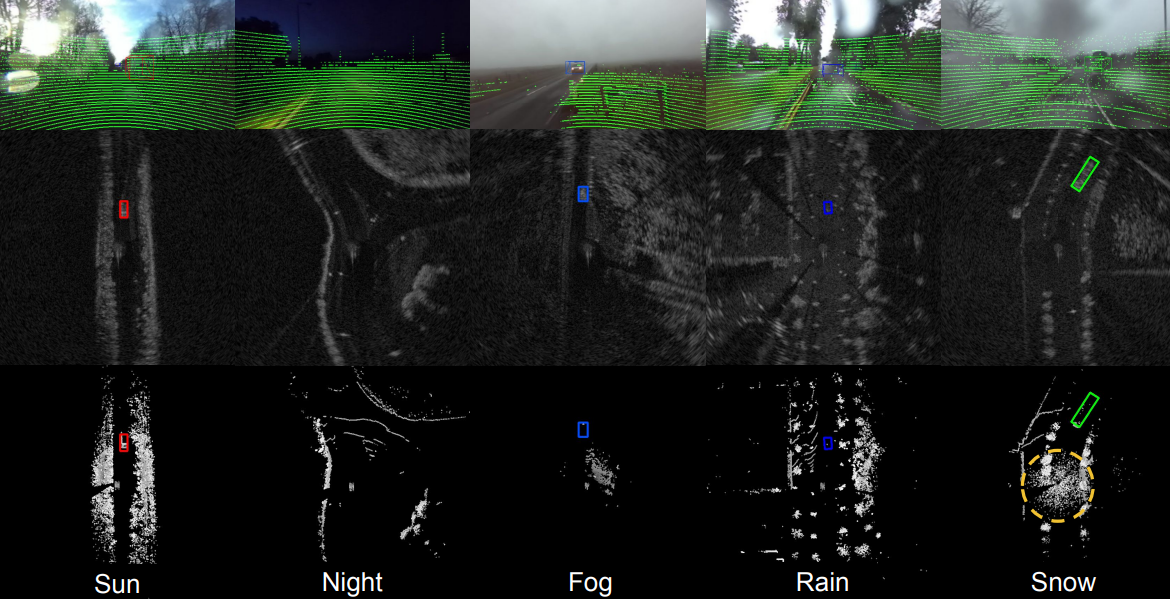
\includegraphics[width=0.9\textwidth]{LidarViews.png}
              \caption{Gradient of Depth Image Around Target Pixel Gives Roughness of the Environment~\cite{https://doi.org/10.48550/arxiv.2010.09076}}
          \end{figure}
\end{itemize}


\subsubsection*{Variables That Effect Stereo Vision Camera:}

\begin{itemize}
    \item Distance:
          
          According to viewing angles and algorithm used to extract depth information from stereo image, there is an uncertainty appears. And this uncertainty increases as distance of the pixel increases. Uncertainty reduces the confidence of the input as it increased.
          
          \begin{figure}[H]
              \centering
              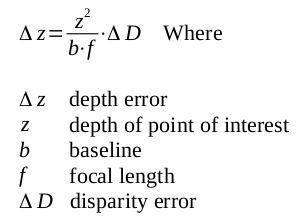
\includegraphics[width=0.4\textwidth]{CamDistance.png}
              \caption{Stereo Camera Depth Error Calculation~\cite{DisparityCalculator, gallup2008variable}}
          \end{figure}
          
    \item Brightness:
          
          The brightness of the environment is important for stereo vision depth estimation. As considering the working principles of the stereo vision depth estimation, there are two frames taken from different angles. First step is matching each pixel of left frame with corresponding pixel in right frame. This step includes computer vision algorithms like Sum of Squared Differences (SSD) and Sum of Absolute Differences (SAD). To perform matching properly, the frames should have well distributed histograms and good contrast values. If there is the brightness of frames are too high or too low, the algorithms cannot match the corresponding pixels.
          
          We can calculate the effect of brightness by observing the histogram of the RGB frames.
    \item Straight and no-Contrast Views:
          
          Like the brightness, the content of the frame is also important. If the frame includes low contrast, straight or similar patterns, the matching algorithms won’t work properly. For example, If the frame includes a flat white wall, the algorithm can not distinguish pixels in different frames. Likewise, if the frame has a periodic pattern like damas pattern, the algorithm also not work well.
          
          In this case we can calculate the effect of straightness by calculating gradient around target pixel in RGB frames.
\end{itemize}

According to these parameters, we will derive confidence generator functions that will calculate a confidence value for each input. By normalizing one of the confidence values will give us $\alpha$ value.

\begin{equation}
    \alpha = \frac{C_{LIDAR}}{C_{LIDAR} + C_{STEREO}}
\end{equation}

\begin{figure}[H]
    \centering
    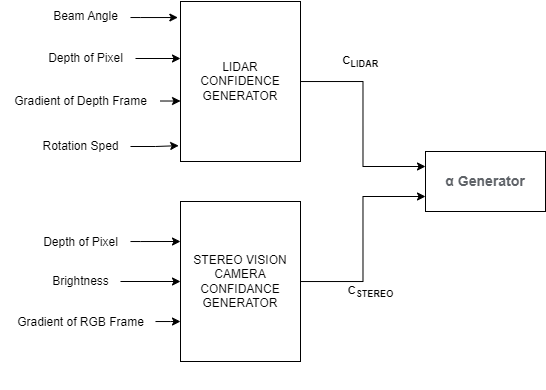
\includegraphics[width=0.9\textwidth]{AlphaFunction.jpeg}
    \caption{Alpha Function for Complementary Filter Enhancement}
\end{figure}

After extracting $\alpha$ value for each pixel of depth frame, we can simply apply complementary filter.

\begin{figure}[H]
    \centering
    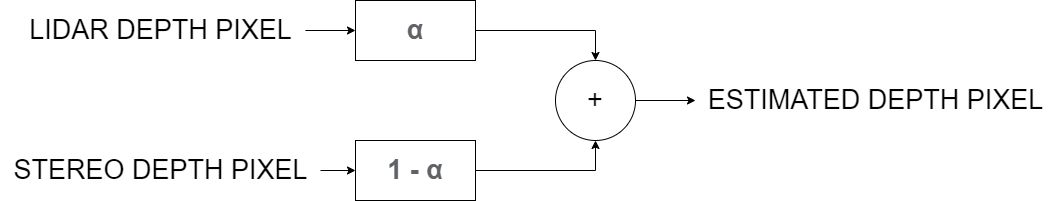
\includegraphics[width=0.9\textwidth]{CompFiltBD.jpeg}
    \caption{Complementary Filter Block Diagram}
\end{figure}


\section{PROTOTYPE}

The prototype developed for this project is a fully ROS-based robot designed to perform sensor fusion and SLAM operations. The primary purpose of building this prototype is to demonstrate the effectiveness of integrating various sensors for accurate and efficient mapping and navigation in an unknown environment. The prototype serves as a platform for testing different sensor fusion algorithms and SLAM techniques to identify the most suitable combination for real-world applications.

The prototype consists of a mobile robotic base equipped with multiple sensors, including LiDAR, camera, inertial measurement unit (IMU), and wheel encoders. These sensors work in tandem to gather data from the environment, which is then processed and combined using sensor fusion algorithms. The fused data is fed into the SLAM system, allowing the robot to construct a map of its surroundings while simultaneously keeping track of its position within that map.

Key features of the prototype include:

\begin{enumerate}
    \item ROS integration: The robot's software architecture is built on the Robot Operating System (ROS), a widely used, flexible framework for robotics development. This allows for easy integration of existing ROS packages and ensures compatibility with a wide range of sensors and algorithms.
          
    \item Sensor fusion: The prototype employs various sensor fusion techniques to combine the data from different sensors, resulting in a more accurate and robust representation of the environment. This helps improve the robot's overall performance in mapping and navigation tasks.
          
    \item SLAM implementation: The prototype integrates state-of-the-art SLAM algorithms to simultaneously localize the robot within the environment and construct a map based on the fused sensor data. This enables the robot to navigate autonomously and efficiently, even in previously unexplored areas.
          
    \item Modular design: The hardware and software components of the prototype are designed to be modular, allowing for easy modification, replacement, and upgrading of individual elements. This ensures that the robot can be easily adapted to accommodate new sensors or algorithms as they become available.
\end{enumerate}

LOAM (Lidar Odometry and Mapping) is a state-of-the-art algorithm for simultaneous localization and mapping (SLAM) that leverages the advantages of lidar sensors. The LOAM algorithm is designed to work in real-time and has been widely adopted in various robotic applications, including autonomous vehicles and drones, due to its robust performance and high accuracy.

The main idea behind LOAM is to separate the point cloud data generated by the lidar sensor into two components: ground points and edge points. Ground points represent the flat surfaces of the environment, while edge points correspond to the sharp features such as corners and edges. By analyzing the relative motion of these two sets of points, LOAM can estimate the robot's pose and build a detailed map of the environment.

LOAM is particularly well-suited for robotic platforms equipped with high-resolution lidar sensors, as it can handle large amounts of data efficiently and maintain accurate localization even in complex environments. Integrating LOAM into the prototype enables the robot to perform SLAM tasks with high precision, making it an ideal choice for the sensor fusion system.

\begin{figure}[h]
    \centering
    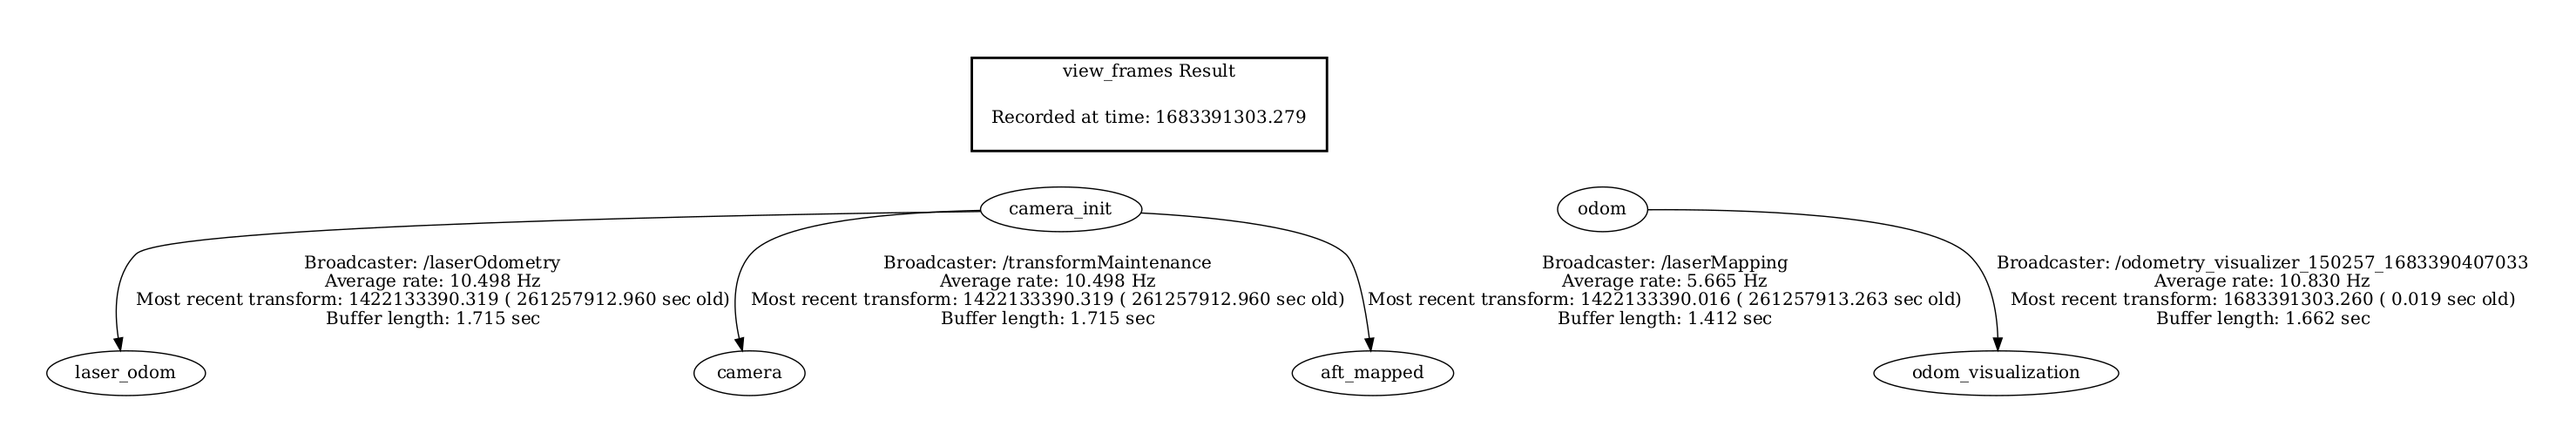
\includegraphics[width=0.9\textwidth]{loam_ros_graph.png}
    \caption{Local Host LOAM ROS Node/Topic Schematic}
\end{figure}

The Robot Operating System (ROS) is a flexible and powerful framework for developing robotic applications, providing a wide range of libraries, tools, and software components for various robotic tasks. Running ROS on a Raspberry Pi (RPI) is an efficient and cost-effective way to create a compact, versatile robotic system that can take advantage of ROS's capabilities.

By utilizing an RPI as the central processing unit for the robot, the system can benefit from the RPI's low power consumption, small form factor, and extensive community support. This allows for a lightweight, portable robotic platform that can be easily extended and customized according to specific application requirements. Moreover, the RPI can run a Linux-based operating system, which is compatible with ROS, making it an ideal choice for integrating ROS into the robot's control system.

Installing and running ROS on an RPI involves setting up the necessary dependencies, configuring the ROS environment, and deploying the desired ROS packages. Once the ROS system is up and running on the RPI, the robot can utilize various ROS functionalities, such as communication between different nodes, sensor data processing, and control algorithms implementation.

Integrating ROS with the RPI enables seamless communication with other hardware components, such as sensors and actuators, through the use of ROS topics, services, and actions. This allows for efficient sensor fusion, SLAM operations, and overall system coordination. The combination of ROS and RPI offers a powerful, compact solution for developing advanced robotic applications while maintaining a low-cost and accessible platform.

\begin{figure}[h]
    \centering
    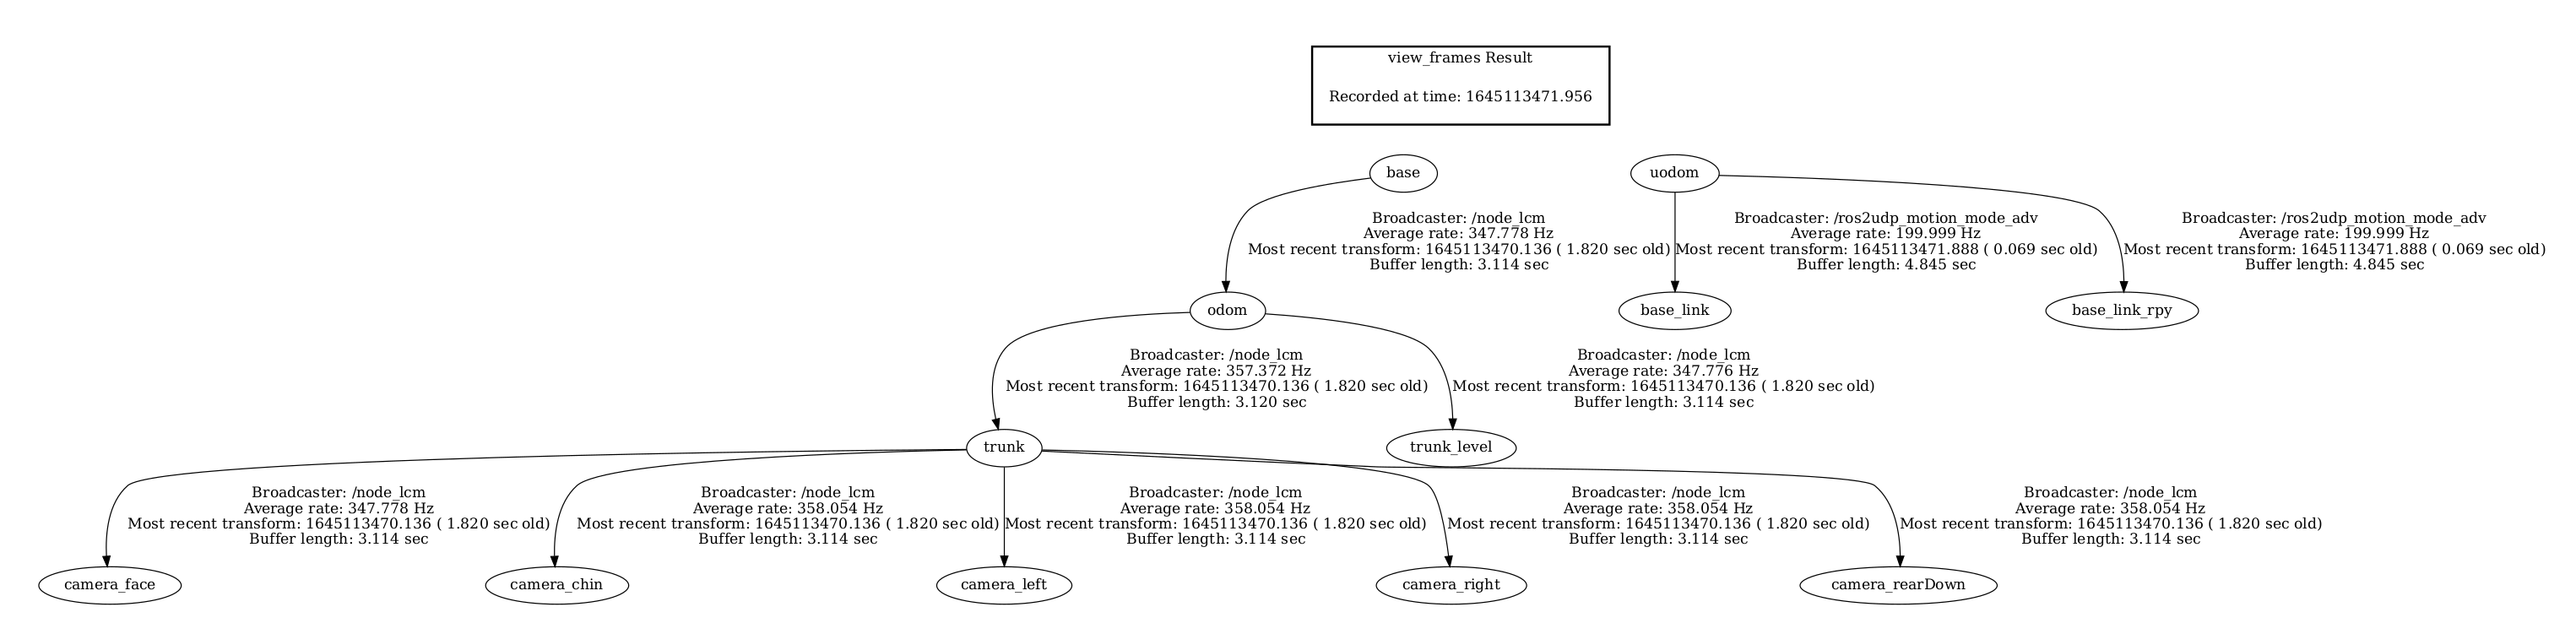
\includegraphics[width=0.9\textwidth]{rpi_ros_graph.png}
    \caption{Legged Robot RPi ROS Node/Topic Schematic}
\end{figure}


\section{DESIGN PROCESS}

The design process of the prototype followed an iterative approach, involving multiple stages of development, testing, and evaluation. This methodology allowed the team to identify shortcomings in the initial design, implement modifications, and continuously improve the prototype's performance. Each iteration focused on addressing specific challenges, refining the sensor fusion techniques, and optimizing the SLAM implementation. In the following subsections, we present the steps of the design process performed in constructing the prototype, including the objectives, testing, results, and evaluation for each iteration.

\subsection{ITERATION 1: INITIAL SENSOR INTEGRATION AND ROS SETUP}

The first iteration aimed to establish a solid foundation for the project by integrating the different sensors and setting up the ROS framework for the robot. The main objectives of this iteration were:

\begin{enumerate}
    \item Selection and integration of appropriate sensors (LiDAR, camera, IMU, and wheel encoders) for the robot.
    \item Installation and configuration of ROS on the robot's embedded computer system.
    \item Setup of the communication infrastructure between the sensors, ROS nodes, and the robot's control system.
\end{enumerate}

In addition to the aforementioned advantages, the integration of the Raspberry Pi (RPI) with the Robot Operating System (ROS) allows for enhanced communication capabilities with micro-ROS systems. Micro-ROS is a lightweight version of ROS specifically designed for microcontrollers, enabling resource-constrained devices to become part of the ROS ecosystem. By incorporating micro-ROS into the system, it becomes possible to extend the functionality and modularity of the robotic platform even further.

The RPI serves as the central communication hub between the ROS nodes and the micro-ROS system. It manages the flow of data between the different subsystems and ensures seamless interaction among the various components of the robot. To facilitate this communication, the RPI is connected to a network switch, which enables efficient data transmission and distribution throughout the system.

The network switch plays a crucial role in the overall performance and reliability of the robotic system. It ensures that all components, including the RPI, micro-ROS nodes, and other connected devices, can exchange information effectively and maintain synchronized operation. By leveraging a network switch in conjunction with the RPI, the system can handle multiple data streams, balance network traffic, and reduce latency, thereby improving the overall performance of the robot.

In summary, the combination of the Raspberry Pi, ROS, micro-ROS, and a network switch provides a powerful and versatile robotic platform. The RPI acts as the central processing unit and communication hub, allowing for efficient coordination between the ROS nodes and micro-ROS systems. The use of a network switch ensures seamless data exchange among the various components of the robot, resulting in a robust, scalable, and high-performance robotic system capable of tackling a wide range of applications.

\begin{figure}[H]
    \centering
    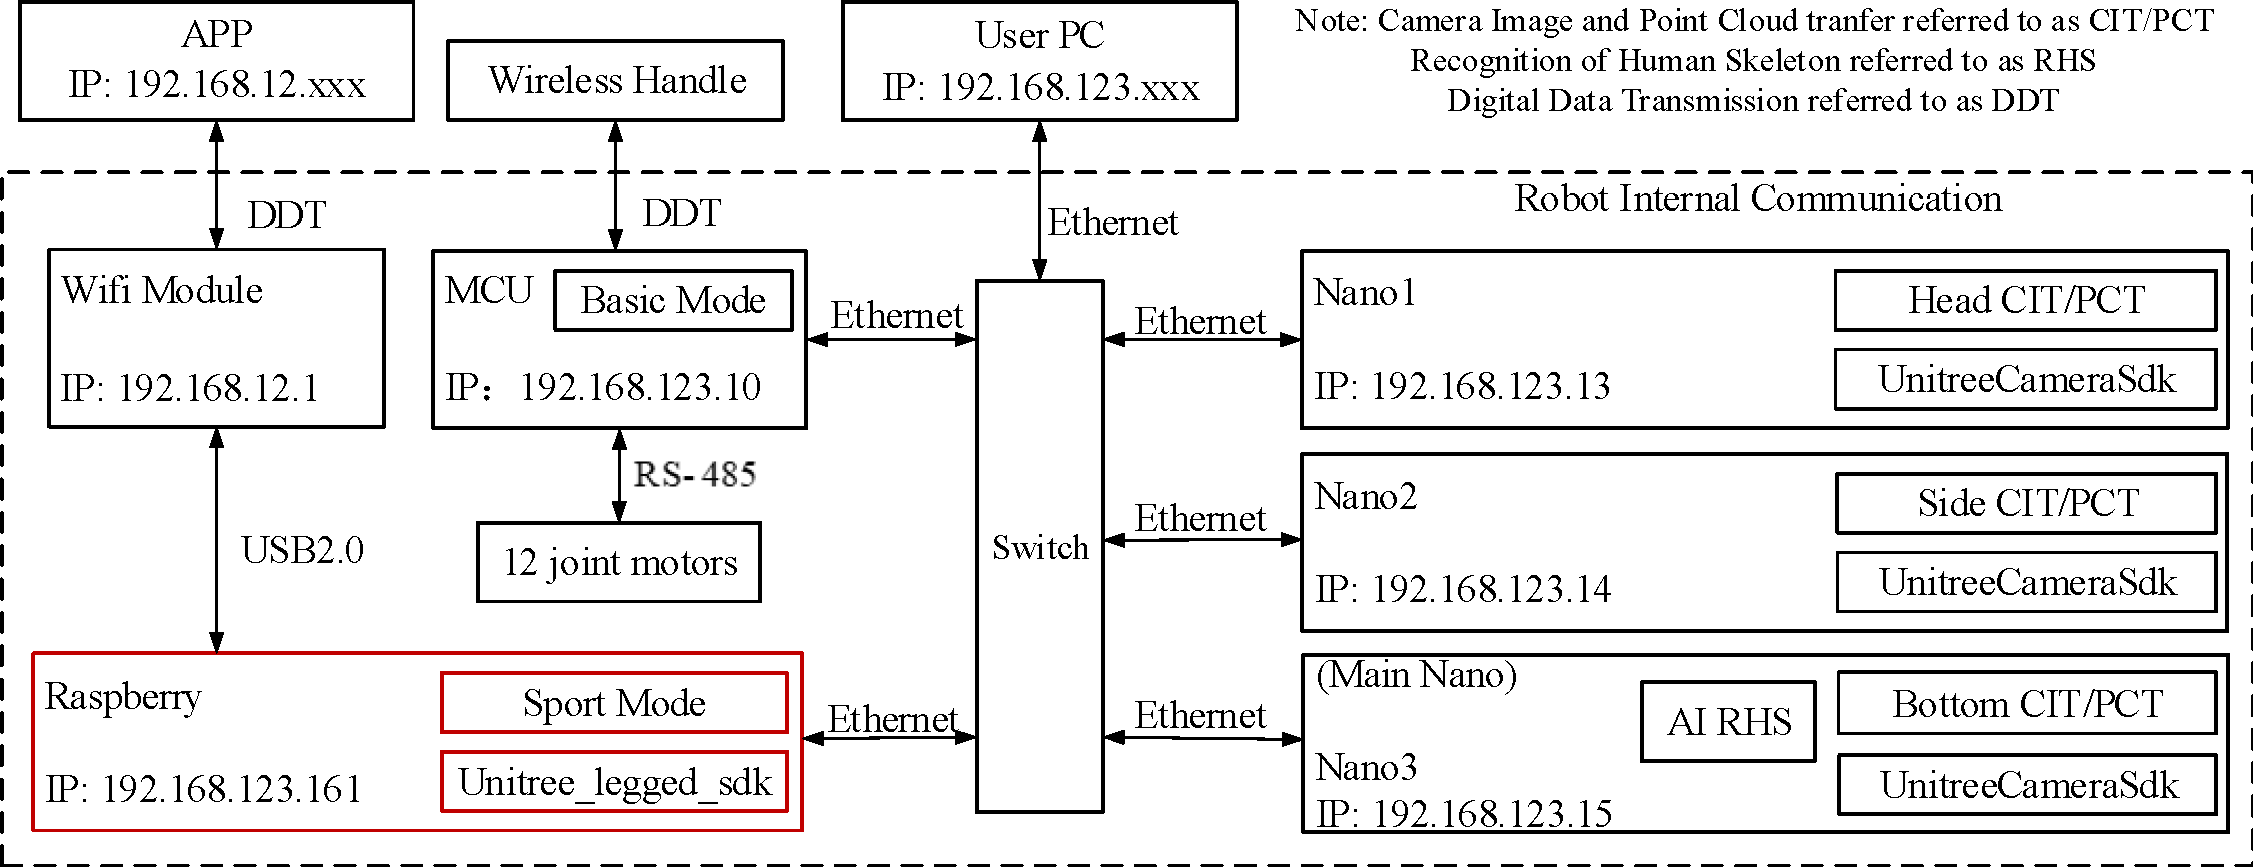
\includegraphics[width=0.9\textwidth]{Go1CommFram_E.png}
    \caption{Infrastructure of the Unitree Go1 Robot}
\end{figure}

\subsubsection{TESTING AND RESULTS}

The robot's hardware and software components were assembled, and the integration of sensors with the ROS framework was tested. The communication between the sensors and ROS nodes was verified using the provided visualization tools (such as RViz) to ensure proper data flow. Preliminary tests were conducted to evaluate the robot's ability to gather data from the environment using the sensors.

\subsubsection{EVALUATION}

The results from the first iteration revealed the successful integration of sensors and the establishment of the ROS environment. However, some issues were identified, such as occasional data loss due to communication bottlenecks and the need for better synchronization between the sensors. These issues were noted and addressed in the subsequent iterations.

\subsection{ITERATION 2: SENSOR FUSION AND SLAM IMPLEMENTATION}

In the second iteration, the focus was on incorporating sensor fusion techniques to combine the data from the different sensors and implementing SLAM algorithms to enable mapping and localization capabilities. The main objectives of this iteration were:

\begin{enumerate}
    \item Development and implementation of sensor fusion algorithms to combine data from the LiDAR, camera, IMU, and wheel encoders.
    \item Selection and integration of a suitable SLAM algorithm for mapping and localization.
    \item Evaluation of the robot's performance in mapping and navigation tasks using the fused sensor data and SLAM system.
\end{enumerate}

\subsubsection{TESTING AND RESULTS}

The sensor fusion algorithms were tested to ensure the proper combination of data from the different sensors. The robot was then deployed in a controlled environment to evaluate its mapping and navigation capabilities using the SLAM system. The resulting maps were compared to the ground truth to assess the accuracy of the robot's localization and mapping.

\subsubsection{EVALUATION}

The results from the second iteration showed significant improvement in the robot's mapping and localization performance. The sensor fusion algorithms effectively combined the data from the different sensors, resulting in a more accurate and robust representation of the environment. However, some challenges remained, such as occasional drift in the robot's position estimation and the need for further optimization of the SLAM algorithm. These issues were addressed in the subsequent iterations.

\subsubsection{ITERATION 3: IMPROVING SENSOR SYNCHRONIZATION AND ROBUSTNESS}

In the third iteration, the team focused on enhancing sensor synchronization and overall system robustness to improve the robot's mapping and localization capabilities. The main objectives of this iteration were:

\begin{enumerate}
    \item Refine sensor synchronization to minimize data loss and inconsistencies between sensor readings.
    \item Implement error handling and recovery mechanisms to increase the system's robustness.
    \item Optimize the SLAM algorithm to reduce drift and improve localization accuracy.
\end{enumerate}

\subsubsection{TESTING AND RESULTS}

The improved sensor synchronization was tested by analyzing the consistency of sensor data and verifying the data alignment using visualization tools. The robot was then deployed in a controlled environment, including areas with challenging conditions, such as uneven terrain, dynamic obstacles, and poor lighting. The robot's performance in mapping, localization, and navigation tasks was assessed, taking into consideration the implemented error handling and recovery mechanisms.

\subsubsection{EVALUATION}

The results of the third iteration showed a notable improvement in sensor synchronization and overall system robustness. The robot was able to handle challenging environmental conditions more effectively and recover from errors more efficiently. However, some areas for further optimization were identified, such as refining the SLAM algorithm for better performance in dynamic environments and enhancing the robot's ability to cope with sensor noise.

\subsection{ITERATION 4: DYNAMIC ENVIRONMENT HANDLING AND NOISE REDUCTION}

The fourth iteration aimed to address the remaining challenges by improving the robot's performance in dynamic environments and reducing the impact of sensor noise. The main objectives of this iteration were:

\begin{enumerate}
    \item Adapt the SLAM algorithm to better handle dynamic environments and moving obstacles.
    \item Implement noise filtering techniques to reduce the impact of sensor noise on the robot's mapping and localization performance.
    \item Evaluate the overall performance of the robot, including its robustness, adaptability, and accuracy in various environmental conditions.
\end{enumerate}

\subsubsection{TESTING AND RESULTS}

The modified SLAM algorithm and noise filtering techniques were tested in multiple environments, including static and dynamic settings. The robot was deployed in a controlled environment with moving obstacles and varying lighting conditions to assess its ability to adapt and maintain accurate mapping and localization performance.

\subsubsection{EVALUATION}

The results from the fourth iteration demonstrated the robot's improved performance in dynamic environments and its enhanced ability to handle sensor noise. The robot was able to maintain accurate mapping and localization despite the presence of moving obstacles and varying environmental conditions. The noise filtering techniques effectively reduced the impact of sensor noise on the robot's performance. With these improvements, the prototype was considered ready for further real-world testing and potential future applications.


\section{FINAL DESIGN}

    \subsection{MEETING THE CONSTRAINTS AND ENGINEERING STANDARDS}

    The final design of our project successfully met the design constraints outlined in the project description. We ensured compliance with the specified economy, environment, manufacturability, and sustainability constraints.

        \subsubsection{Economy}

        Throughout the project, we maintained strict control over costs to meet the project's economic constraints. By leveraging the Unitree Go1 Edu robot's internal Nvidia Jetson Nano 4GB devices for computing power, we were able to reduce expenses compared to using external computing units. Additionally, the use of readily available sensors and components helped keep the overall costs within budget.

        \subsubsection{Environment}

        The environmental impact of our project was considered at various stages of development. We focused on using battery-powered systems, minimizing power consumption, and adhering to legal regulations regarding radiation and noise pollution. By selecting energy-efficient components and optimizing algorithms, we aimed to reduce the ecological footprint of the robotic platform.

        \subsubsection{Manufacturability}

        The prototype design prioritized manufacturability by utilizing readily available products and components. This approach minimized the need for high-level manufacturing technologies and complex assembly processes. The modular design of the robot and its compatibility with existing ROS packages also facilitated the integration of different hardware and software components.

        \subsubsection{Sustainability}

        Our project aimed to establish a sustainable foundation for future developments. By emphasizing the mathematical foundations, software abstractions, and comprehensive engineering solutions, we laid the groundwork for future advancements and upgrades. The modular design of the robot, adherence to engineering standards, and consideration of safety measures ensured the long-term sustainability and reliability of the robotic platform.

        The project also met the engineering standards and best practices to ensure the reliability, maintainability, and safety of the robotic platform. We followed software engineering principles, such as modular design, code documentation, version control, and code reviews. The adoption of the ROS framework provided a standardized and modular approach to software development, enhancing interoperability and code reusability. Safety measures were implemented to prevent potential hazards, and documentation and reporting were maintained throughout the project to ensure traceability and knowledge dissemination.

    \subsection{COST ANALYSIS}

    The cost analysis of our project includes both initial costs and potential future costs for production and maintenance. The initial costs include the purchase of components and materials required for building the prototype, while the future costs involve scaling up production and maintaining the robotic platform.

        \subsubsection{Initial Costs}

        The initial costs for our project primarily consisted of the Unitree Go1 Edu robot and additional sensors. The Unitree Go1 Edu robot, including its embedded computing units and sensors, had a cost of approximately \$ 18,000. The cost breakdown of the additional sensors used in the project is as follows:
            
        \begin{itemize}
            \item LiDAR: Velodyne 80-VLP-16-A 3D LiDAR - \$ 2500.
            \item Camera: StereoLabs ZED Stereo Camera - \$ 1000.
        \end{itemize}
        
        The total initial cost of the prototype, including the robot and additional sensors, amounted to approximately \$ 22,500.

        \subsubsection{Future Costs}

        Future costs for production and maintenance may vary depending on the scale of deployment and specific application requirements. Some potential future costs to consider include:

        \begin{itemize}
            \item Production Costs: Scaling up production would involve the cost of manufacturing additional robotic platforms, including the necessary components and assembly processes. These costs would depend on the production volume and any customization required for specific applications.
            \item Maintenance Costs: Maintenance costs would include periodic hardware inspections, software updates, and component replacements. The costs would depend on the frequency and complexity of maintenance tasks, as well as any warranty or support agreements.
            \item Upgrades and Expansion: As technology advances and new sensors or algorithms become available, there may be additional costs associated with upgrading or expanding the capabilities of the robotic platform. These costs would depend on the specific upgrades and their integration complexity.
        \end{itemize}

        It is important to note that the costs mentioned above are estimates based on current market prices and may vary depending on factors such as location, supplier, and future market conditions.

        \subsubsection{Cost-Benefit Analysis}

        While the cost of the project may be significant, it is essential to consider the potential benefits and applications of the developed robotic platform. The integration of sensor fusion, SLAM techniques, and cloud computing provides opportunities for various industries, including autonomous vehicles, UAVs, augmented reality devices, and 3D modeling. The accuracy and efficiency of the depth estimation and mapping capabilities make the platform valuable for navigation in unknown environments. The scalability and modularity of the design also allow for future upgrades and customization, ensuring long-term usability and adaptability.

        The cost-benefit analysis should take into account the potential economic, environmental, and societal impact of deploying such a robotic platform. While the costs may be higher initially, the benefits derived from improved navigation, mapping, and perception capabilities can outweigh the expenses in various domains. Furthermore, the sustainability and modularity of the design contribute to long-term cost savings by enabling upgrades and maintenance rather than complete system replacements.

    \subsection{SUMMARY}

    The final design of our project successfully met the specified design constraints, including economic, environmental, manufacturability, and sustainability considerations. The adherence to engineering standards ensured the reliability, maintainability, and safety of the robotic platform. The cost analysis provided an overview of the initial costs and potential future costs for production, maintenance, and upgrades. By considering the potential benefits and applications of the developed robotic platform, the cost-benefit analysis demonstrates the value and long-term viability of the project. Overall, the final design represents a comprehensive and practical solution for sensor fusion, SLAM implementation, and cloud computing integration in autonomous robotic systems.

\section{TEAM WORK}

Teamwork is an essential aspect of any successful project, and this project is no exception. Our team is composed of multiple members with different backgrounds, expertise, and skills, working together to achieve a common goal. To ensure effective collaboration and communication among team members, we have chosen to use Github as our primary source control and project management platform. This allows us to easily share code, track changes, and collaborate on different parts of the project.

In addition to Github, we are also using MATLAB, Python, and the Robot Operating System (ROS) environment for our project. These tools provide us with the necessary functionality and flexibility to implement and test our sensor fusion algorithm. MATLAB, in particular, is useful for prototyping and simulating our algorithm, while Python and ROS provide us with the ability to implement and test our algorithm on real-world systems.

We also keep a logbook during the project which contains our daily progress, issues encountered, and solutions implemented. This logbook acts as a reference for team members and helps keep track of the project's history and progress. Keeping a logbook is a best practice in project management, as it helps to stay organized, keep track of progress, and document any issues that may arise.

Other papers in the field also highlighted the importance of team work, communication, and collaboration in the development of sensor fusion algorithms. For example, in their paper on sensor fusion for mobile robots, authors underline that the development of a sensor fusion algorithm is a complex task that requires a multidisciplinary team with expertise in various fields such as robotics, control systems, and computer vision. They also point out that effective communication and collaboration among team members is crucial to the success of the project.

According to \cite{daniilidis2001sensor}, sensor fusion is a complex task that has been extensively studied and is widely used in various applications. In \cite{durrant2006simultaneous}, it was stated that simultaneous localization and mapping (SLAM) is an important problem in the field of robotics that requires the integration of sensor data through sensor fusion. Additionally, in \cite{silva2020edge} the authors proposed to use edge preservation methods to increase the performance of depth map filtering for stereo vision, which can be useful for our sensor fusion algorithm.

In conclusion, effective teamwork is crucial to the success of this project, and we are utilizing a variety of tools and best practices to ensure that our team can work together effectively. Our use of Github, MATLAB, Python, and the ROS environment, as well as our logbook and regular team meetings, will help us to stay organized and work effectively together to achieve our goals.

\section{COMMENTS AND CONCLUSIONS}

In conclusion, sensor fusion is an essential component of modern technology that is used to sense and augment the environment. Our proposed project aims to develop a sensor fusion algorithm for extracting depth information using data from living organisms, specifically studying the way in which zebra fish process sensor data to produce depth information. We plan to use a legged robot for the system and cloud computing for high computing power requirements. The preliminary design of the project includes using the ZED stereo camera and Velodyne 3D LiDAR as sensors and implementing a complementary filter algorithm to fuse the depth information from the two sensors, with edge preservation methods being used as an aid to the main algorithm to increase performance.

Effective teamwork and collaboration among team members are crucial to the success of this project, and we are utilizing a variety of tools and best practices such as Github, MATLAB, Python, the Robot Operating System (ROS) environment, and a logbook to ensure that our team can work together effectively. We also have been studying the sensor fusion and alternative methodologies to implement it correctly to serve the main purpose of sensor fusion, that is reliable odometry data extraction.

In future work, we plan to improve the sensor fusion algorithm by incorporating data from the zebra fish, optimize the resolution and data rates, and test the algorithm on a legged robot with cloud computing. Additionally, we plan to implement the sensor fusion algorithm on an autonomous SLAM robot to demonstrate the usefulness of the depth information in real-world applications.

The preliminary design of our sensor fusion algorithm includes the use of the ZED stereo camera and Velodyne 3D LiDAR sensors as they are well-documented, have a large community, and are easier to use and access resources than the internal sensors of the legged robot. The sensor fusion algorithm chosen for the preliminary design is a complementary filter, which is a simple and low-performance algorithm, but it can be improved by using edge preservation methods to increase the sensor fusion performance. We have also considered the different properties, advantages, and disadvantages of the sensors to optimize the sensor fusion algorithm. The stereo vision camera and 3D lidar have different viewing angles, data formats, and sample rates, thus we have to match them by reducing the viewing angle of the 3D lidar, upsampling the lidar data, converting it to cartesian form, and using dynamic Papoulis-Gerchberg algorithm to augment the lidar data. We also aim to optimize resolution and data rates in the future work to increase the quality of the point clouds and reduce the computational effort.

In addition to the previous conclusions, it is worth noting that the preliminary design of our sensor fusion algorithm was realized using the MATLAB programming environment. This choice was made because of the wide range of tools and functions available in MATLAB for image processing and sensor data manipulation, as well as its user-friendly interface and compatibility with other programming languages such as Python and C++.

By using MATLAB, we were able to effectively implement the sensor fusion algorithm, including the complementary filter, edge preservation methods, and dynamic Papoulis-Gerchberg algorithm. We also were able to test the algorithm with sample data and evaluate its performance.

It is important to note that while the preliminary design has been realized in MATLAB, we plan to implement the final version of the sensor fusion algorithm in an appropriate programming environment for the legged robot, such as ROS, to ensure the compatibility and efficiency of the algorithm in the real-world application.

\addcontentsline{toc}{section}{REFERENCES}
\bibliographystyle{plain}
\bibliography{refs}
\end{document}